\documentclass[a4j]{jarticle}
\usepackage[dvipdfmx]{graphicx,color}
\usepackage{verbatim}
\usepackage{ascmac}
\usepackage{url}
\usepackage{listings,jlistings}
\usepackage{color}
%\setlength{\marginparwidth}{20mm}%% 傍注欄の横幅の設定

\input{/home/ryousuke/listings_temp.tex}

\title{情報科学プロジェクト実験レポート課題}
\author{S142063 佐藤涼亮}

\begin{document}
\maketitle
\centerline{\LARGE \underline{Ajax(Asynchronous JavaScript + XML)}}
\section{課題の内容}
{\large \underline{XMLHttpRequestによるJavaScriptからのHTTPの制御}}
\subsection{要点}
\begin{itemize}
\item Ajaxの技術を用いて、ページリロードをしないWebプログラムの実装
\item C++プログラムをCGIプログラムとして実装
\item 入力されたデータをデータベースに格納
\end{itemize}
\section{プログラムの説明}
入力画面では、
郵便番号、住所、氏名、年齢、性別の入力欄を設け、
データの入力を求める。
Ajaxにより郵便番号7桁から住所入力の補助を行う。
郵便番号の入力欄は、7桁を最大とし、
7桁入力された時点でCGIプログラムにより、
入力された郵便番号の住所を検索し、住所の欄に結果を入れる。
消去ボタンと送るボタンを設け、消去ボタンはformのリセット、
送るボタンは、CGIプログラムにformを送信し、確認画面の表示をする。
未入力の欄があれば入力を促すダイアログを表示する。

確認画面では、
入力画面で入力されたデータをテーブル方式で表示し、
確認を求める。
編集ボタンと送るボタンを設け、編集ボタンはデータをそのままに入力画面に戻り、
送るボタンはデータをCGIプログラムに送り、データをデータベースに格納する。
その後、最終画面を表示する。

CGIプログラムは一つにまとめ、行う動作の判別のために、
シリアライズされたformの末尾にflagを追加し渡すことで判別を可能にした。

\newpage
Webサーバ上のディレクトリ情報は以下のとおりである。
\begin{verbatim}
                    html/
                    ├── cgi/
                    │  ├── data.cgi
                    │  ├── db/
                    │  │  ├── data.db
                    │  │  └── tokyo.db
                    │  └── src/
                    │     └── data.cpp
                    ├── script.js
                    └── data.html
\end{verbatim}


データを格納するデータベース(data.db)のテーブル、スキーマは以下の通りである。
\begin{screen}
\begin{verbatim}
sqlite> .table
data
sqlite> .schema
CREATE TABLE data
(num text,addr text,name text,age int,gender text);
\end{verbatim}
\end{screen}

\subsection{目的}
XMLHttpRequestによるJavaScriptからのHTTPの制御

\subsection{方法}
Ajaxの技術を用いて、ページのリロードを行わないWebプログラムの実装

\subsection{結果}

\begin{center}
初期状態
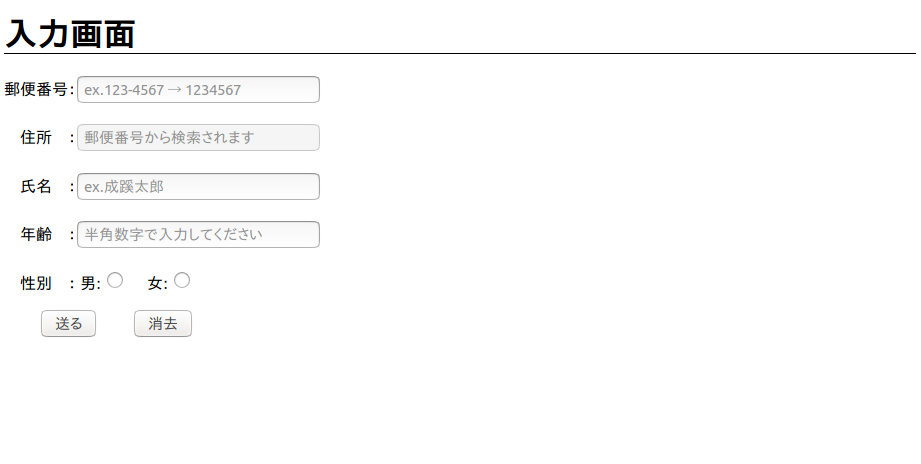
\includegraphics[width=15cm]{result/result1.png}\\
すべての項目を入力せずに送るボタンを押すと注意される。\\
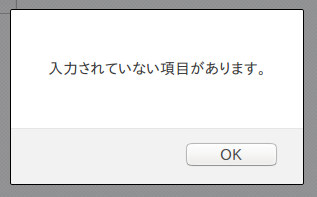
\includegraphics[width=8cm]{result/result2.png}

{\LARGE↓}

すべての項目を入力する
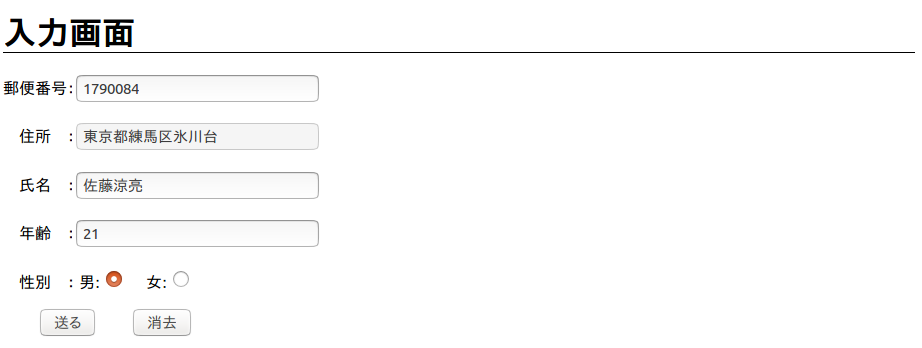
\includegraphics[width=15cm]{result/result3.png}

{\LARGE↓}

入力画面から送るボタンを押すと確認画面が表示される
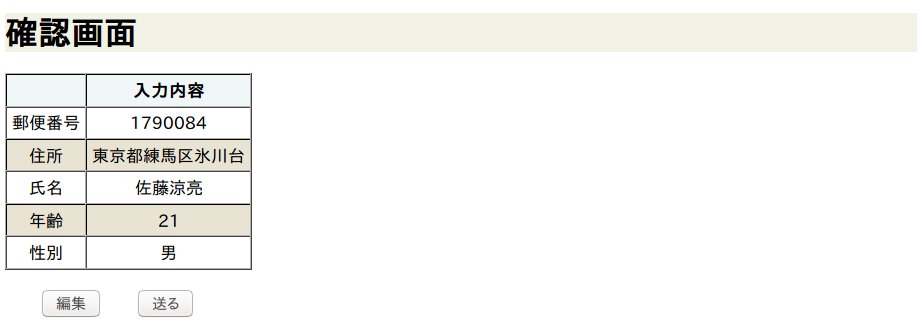
\includegraphics[width=15cm]{result/result4.png}
(ここで編集ボタンを押すと入力画面に戻る)

{\LARGE↓}

確認画面から送るボタンを押すと最終画面が表示され終了する

\includegraphics[width=8cm]{result/result5.png}
\end{center}

\subsection{考察}
実行前のデータベースの状態は以下のとおりである。
\begin{screen}
\begin{verbatim}
sqlite> select * from data;
sqlite>
\end{verbatim}
\end{screen}\\

実行後、データベースは以下のとおりになる。
\begin{screen}
\begin{verbatim}
sqlite> select * from data;
1790084|東京都練馬区氷川台|佐藤涼亮|21|男
sqlite> 
\end{verbatim}
\end{screen}
これらより、データの格納は成功し、ページのリロードも行われなかったことから、
期待通りの結果が得られた。
\section{感想}
前回に引き続きC++プログラムによるCGIプログラムとHTMLに加え、
今回はJavaScriptプログラムを加えた、
XMLHttpRequestを用いたAjaxプログラムについて学習した。
非同期通信により、サーバの処理待ちを必要とせず、
ページ遷移することなく高速で画面の切り替えが可能であり、
ユーザの動作を止めることなくスムーズな簡単なページが実現できるようになった。
簡単なWebページではあるが、普段自分が閲覧、利用しているようなWebページが、
自分の手で制作することができて感動した。
さらに学習をすることで、複雑なWebページを理解できるようになりたい。

\section{プログラム}
\lstinputlisting[caption=data.html,language=HTML5]{data.html}
\lstinputlisting[caption=script.js,language=HTML5]{script.js}
\lstinputlisting[caption=data.cpp,language=C++]{data.cpp}

\end{document}
